% Положения теории графов, используемые в разделе.
\subsection{Положения теории графов, используемые в главе}

Рассмотрим кубический плоский граф и вопросы его реберных раскрасок.
При этом, наряду с доказательствами существования самих раскрасок будем рассматривать алгоритмы построения этих раскрасок.
Сначала рассмотрим наиболее тривиальное утверждение.

%------------------------------------------------------------------------------------------------------

\begin{lemma}\label{lem:text_3_graph_prim_coloring5}
Кубический граф допускает реберную раскраску в $5$ цветов, и эта раскраска может быть построена с линейной сложностью по количеству ребер.
\end{lemma}
Для построения требуемой раскраски достаточно последовательно перебрать все ребра.
Так как для каждого ребра существует ровно $4$ смежные ребра, то из пяти цветов всегда можно выбрать цвет, в который не покрашено ни одно из этих смежных ребер.
Таким образом, раскраска строится за один проход по всем ребрам, то есть с линейной сложностью.
$\blacksquare$\\

%------------------------------------------------------------------------------------------------------

В лемме~\ref{lem:text_3_graph_prim_coloring5} не использовалась планарность графа, а количество цветов явно избыточно.
Согласно теореме Визинга \cite{Vizing1964}, \cite{Vizing1965} кубический граф допускает реберную раскраску в $4$ цвета.
Однако, теорема Визинга также не использует планарность графа, и алгоритм, построенный исходя из доказательства, будет иметь сложность, выше линейной по количеству ребер \cite{Soifer2009}.
Приведем альтернативное доказательство с использованием планарности графа и более низкой сложностью алгоритма построения реберной раскраски в $4$ цвета.

\begin{lemma}\label{lem:text_3_graph_prim_coloring4}
Кубический граф допускает реберную раскраску в $4$ цвета, и эта раскраска может быть построена с линейной сложностью по количеству ребер.
\end{lemma}

Доказательство существования раскраски будем проводить по индукции по количеству вершин графа.
База индукции: кубический граф с минимальным количеством вершин это $K_4$.
Для этого графа утвержление очевидно.

Предположим, что утверждение теоремы верно для всех кубических графов с порядок которых изменяется от $4$ до $n - 2$ (отметим, что порядок кубического графа не может быть нечетным).

Рассмотрим кубический планарный граф, с множеством вершин $V$ ($n = |V| = \nu$), множеством ребер $E$ ($|E| = \varepsilon$) и множеством граней $F$ ($|F| = \zeta$).
При этом внешнюю область вокруг графа также считаем гранью (рассматриваем граф, расположенный на сфере).
Также через $\zeta_i$ обозначим количество граней, содержашей ровно $i \ge 3$ вершин (в этом случае будем говорить, что грань имеет размер $i$).
\begin{equation}
	\zeta = \sum_{i = 3}^{\infty}{\zeta_i}.
\end{equation}
Рассмотрим соотношения, выполняемые для этого графа.

Так как степень каждой вершины равна $3$, то лемма о рукопожатиях для этого графа приобретает вид
\begin{equation}
	3 \nu = 2 \varepsilon.
\end{equation}

Так как каждое ребро входит ровно в две грани, то верно соотношение
\begin{equation}
	2 \varepsilon = \sum_{i = 3}^{\infty}{i \zeta_i}.
\end{equation}

Наконец, для рассматриваемого графа выполняется соотношение Эйлера $\nu + \zeta - \varepsilon = 2$.
Подставив в соотношение Эйлера выражения для $\nu$, $\zeta$ и $\varepsilon$ получим
\begin{equation}
	2 \cdot 2\varepsilon + 6 \sum_{i = 3}^{\infty}{\zeta_i} - 3 \cdot 2\varepsilon = 12
\end{equation}
\begin{equation}
	6 \sum_{i = 3}^{\infty}{\zeta_i} - \sum_{i = 3}^{\infty}{i \zeta_i} = 12
\end{equation}
\begin{equation}\label{eqn:text_3_graph_prim_euler}
	\sum_{i = 3}^{\infty}{(6 - i) \zeta_i} = 12
\end{equation}

Из \eqref{eqn:text_3_graph_prim_euler} видно, что в рассматриваемом графе найдется грань размера $3$, $4$ или $5$.
Рассмотрим каждый этих случаев отдельно.

Случай 1. Сначала рассмотрим случай наличия в графе гамака, состоящего из двух треугольных граней, как показано на рис.~\ref{fig:text_3_graph_prim_coloring4_gamak} слева.

\begin{figure}[ht]
\centering
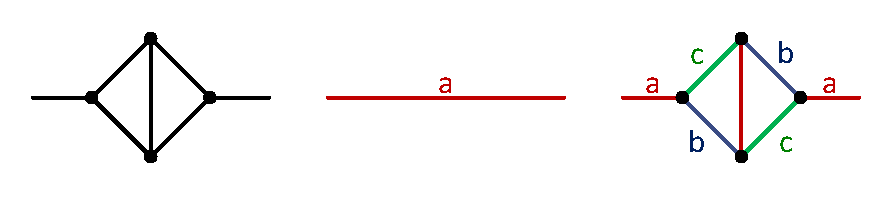
\includegraphics[width=1.0\textwidth]{./pics/text_3_graph_prim/coloring4_gamak.pdf}
\singlespacing
\captionstyle{center}\caption{Случай наличия в графе гамака из двух треугольных граней.}
\label{fig:text_3_graph_prim_coloring4_gamak}
\end{figure}

Стянув гамак в одно ребро (рис.~\ref{fig:text_3_graph_prim_coloring4_gamak} в центре), получим граф с $n - 4$ вершинами, ребра которого могут быть раскрашены в 4 цвета по предположению индукции.
Тогда по этой раскраске не представляется сложным раскрасить исходный граф, как показано на рис.~\ref{fig:text_3_graph_prim_coloring4_gamak} справа.

Случай 2. В графе нет гамаков, состоящих из двух треугольных граней, но найдется треугольная грань (см. рис.~\ref{fig:text_3_graph_prim_coloring4_face3} слева).

\begin{figure}[ht]
\centering
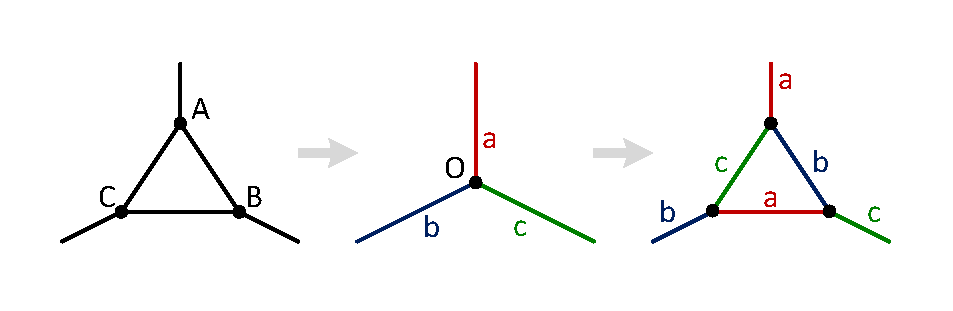
\includegraphics[width=1.0\textwidth]{./pics/text_3_graph_prim/coloring4_face3.pdf}
\singlespacing
\captionstyle{center}\caption{Случай наличия в графе треугольной грани.}
\label{fig:text_3_graph_prim_coloring4_face3}
\end{figure}

Стянем треугольную грань $ABC$ в точку $O$, как показано на рис.~\ref{fig:text_3_graph_prim_coloring4_face3} в центре.
Так как в графе не было гамаков, состоящих из двух треугольных граней, то у грани $ABC$ не было соседних треугольных граней по ребру, а значит при стягивании $ABC \rightarrow O$ ни одна грань кроме $ABC$ не выродилась.
Это значит, что мы получили плоский кубический граф с $n - 2$ вершинами, ребра которого могут быть раскрашены в 4 цвета по предположению индукции.
Тогда по этой раскраске можно построить раскраску исходного графа, как показано на рис.~\ref{fig:text_3_graph_prim_coloring4_face3} справа.

Случай 3. В графе нет треугольных граней, но найдется четырехугольная грань (см. рис.~\ref{fig:text_3_graph_prim_coloring4_face4} слева).

\begin{figure}[ht]
\centering
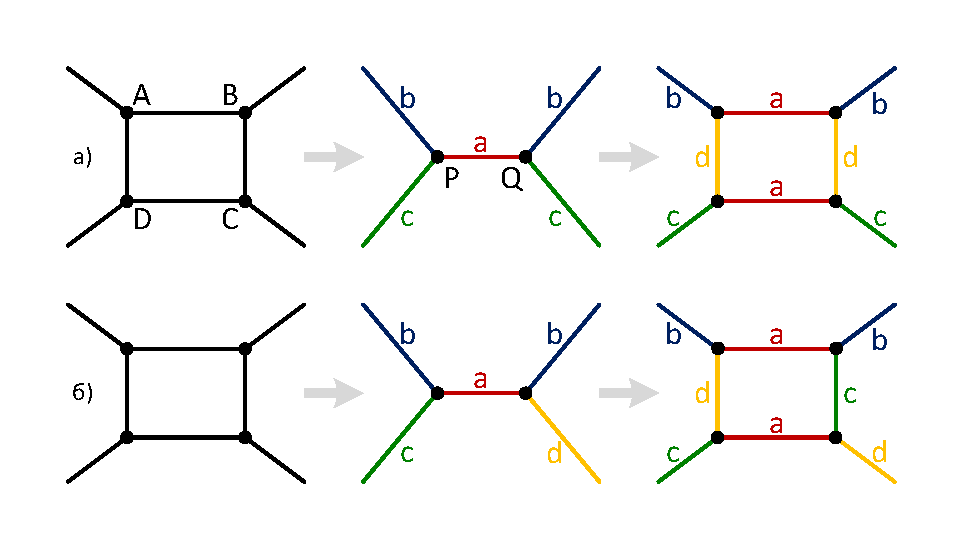
\includegraphics[width=1.0\textwidth]{./pics/text_3_graph_prim/coloring4_face4.pdf}
\singlespacing
\captionstyle{center}\caption{Случай наличия в графе четырехугольной грани.}
\label{fig:text_3_graph_prim_coloring4_face4}
\end{figure}

Рассмотрим четырехугольную грань $ABCD$.
Выполним стягивание ребер $AD \rightarrow P$, $BC \rightarrow Q$.
Так как в графе не было треугольных граней, то при стягивании выродилась только грань $ABCD$.
Мы получили плоский кубический граф с $n - 2$ вершинами, ребра которого могут быть раскрашены в 4 цвета по предположению индукции.
По этой раскраске построим раскраску исходного графа.
Для этого перенесем цвета всех ребер (кроме $PQ$) на исходный граф, непокрашенными останутся только ребра цикла $A-B-C-D$.
Пусть $\gamma(PQ) = a$.
Если для покраски остальных 4 ребер, инцидентных вершинам $P$ и $Q$, были использованы только 2 цвета ($b$ и $c$), то исходный граф можно покрасить в 4 цвета, покрасив ребра цикла $A-B-C-D$ в цвета $a$ и $d$ (см. рис.~\ref{fig:text_3_graph_prim_coloring4_face4} сверху).
Если для покраски остальных 4 ребер, инцидентных вершинам $P$ и $Q$, были использованы все оставшиеся три цвета ($b$, $c$ и $d$), то одним из этих цветов было покрашено 2 ребра (пусть это будет цвет $b$), а двумя другими цветами -- по одному ребру (см. рис.~\ref{fig:text_3_graph_prim_coloring4_face4} снизу).
В этом случае раскрасим ребра цикла $A-B-C-D$ в цвета $a$, $c$, $d$ следующим образом.
К циклу $A-B-C-D$ примыкает одно ребро цвета $c$, оно смежно двум ребрам этого цикла (которые являются смежными), которые не могут быть покрашены с цвет $c$.
То есть в циикле $A-B-C-D$ найдется пара смежных ребер, одно из которых может быть покрашено в цвет $c$ (обозначим эту пару $p_c$).
Аналогично, в цикле $A-B-C-D$ найдется пара смежных ребер, одно из которых может быть покрашено в цвет $d$ (обозначим эту пару $p_d$).
Вне зависимости от того пересекаются ли $p_c$ и $p_d$, в цикле $A-B-C-D$ можно найти такие несмежные ребра $e_c$ и $e_d$, что $e_c \in p_c$, $e_d \in p_d$.
Тогда покрасим ребро $e_c$ в цвет $c$, ребро $e_d$ -- в цвет $d$, а остальные два несмежных ребра -- в цвет $a$ (см. рис.~\ref{fig:text_3_graph_prim_coloring4_face4} снизу справа).

Случай 4. В графе нет треугольных и четырехугольных граней, но найдется пятиугольная грань.

\begin{figure}[ht]
\centering
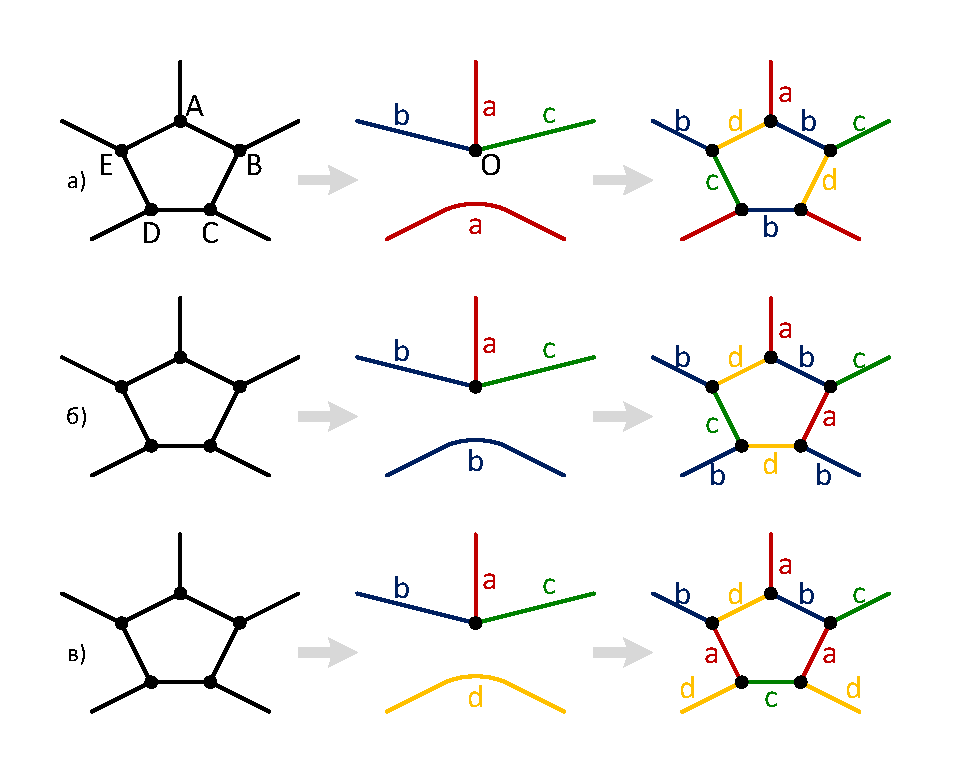
\includegraphics[width=1.0\textwidth]{./pics/text_3_graph_prim/coloring4_face5.pdf}
\singlespacing
\captionstyle{center}\caption{Случай наличия в графе пятиугольной грани.}
\label{fig:text_3_graph_prim_coloring4_face5}
\end{figure}

Рассмотрим пятиугольную грань $ABCDE$.
Удалим ребра $ED$ и $BC$.
Стянем вершины $E$, $A$, $B$ в одну вершину $O$.
Стянем вершины $D$, $C$ в одну вершину степени 2, которую сразу удалим, соединим инцидентные ей ребра в одно $D'C'$ (см. рис.~\ref{fig:text_3_graph_prim_coloring4_face5}).
Так как в графе отсутствовали треугольные грани, то ни одна грань кроме $ABCDE$ не выродилась.
Таким образом, мы получили граф с $n - 4$ вершинами, ребра которого могут быть раскрашены в 4 цвета.
По этой раскраске построим раскраску исходного графа.
Для этого перенесем цвета всех ребер на исходный граф, непокрашенными останутся только ребра цикла $A-B-C-D-E$.
Если для покраски ребер $OA'$, $OE'$, $OB'$, $D'C'$ были использованы три цвета ($a$, $b$, $c$), то без ограничения общности можно рассмотреть только два варианта раскраски: $\gamma(D'C') = \gamma(OA')$ (см. рис.~\ref{fig:text_3_graph_prim_coloring4_face5}, а) и $\gamma(D'C') \ne \gamma(OA')$ (см. рис.~\ref{fig:text_3_graph_prim_coloring4_face5}, б). 
Случай же, когда для покраски ребер $OA'$, $OE'$, $OB'$, $D'C'$ были использованы все 4 цвета, представлен на рис.~\ref{fig:text_3_graph_prim_coloring4_face5}, в.
Во всех трех случаях ребра цикла $A-B-C-D-E$ могут быть раскрашены с сохранением правильной реберной раскраски в 4 цвета.

Рассмотрев все возможные случаи нам удалось раскрасить текущий граф с $n$ вершинами в 4 цвета, опираясь на реберные раскраски графов меньших порядков.
Таким образом, предположение индукции верно, и плоский кубический граф может быть раскрашен в 4 цвета.

Доказательство существования раскраски конструктивно, алгоритм раскраски может быть построен путем стягивания гамаков и граней графа вплоть до графов минимального размера, с последующим восстановлением и посторением раскраски.
Каждое действие по стягиванию и построению раскраски текущего графа на основе раскраске графа меньшего порядка, осуществляется за количество действий $O(1)$.
Каждое стягивание уменьшает количество граней графа хотя бы на 1, таким образом общая сложность алгоритма $O(\zeta)$, что для кубического графа равносильно $O(\nu)$ или $O(\varepsilon)$.
$\blacksquare$\\

%------------------------------------------------------------------------------------------------------

Утверждение о возможности раскраски ребер плоского кубического графа в три цвета является горазд более сильным, оно верно для плоских кубических графов без мостов и равносильно задаче о четырех красках \cite{Soifer2009,Tait1880}.

%------------------------------------------------------------------------------------------------------

%\begin{lemma}\label{lem:text_3_graph_prim_cycle2_inner_space}
%Количество вершин графа, расположенных внутри двухцветного цикла, а также количество ребер, направленных внутрь двухцветного цикла, четные.
%\end{lemma}

%\begin{figure}[ht]
%\centering
%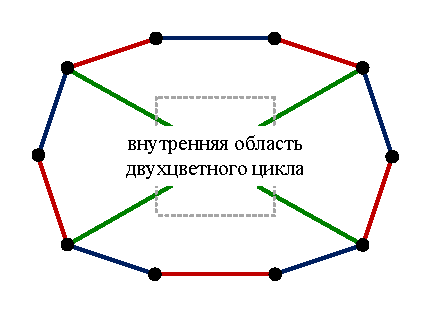
\includegraphics[width=0.5\textwidth]{./pics/text_3_graph_prim/cycle2_inner_space.pdf}
%\singlespacing
%\captionstyle{center}\caption{Структура внутренней области двухцветного цикла.}
%\label{fig:text_3_graph_prim_cycle2_inner_space}
%\end{figure}

%На рис.~\ref{fig:text_3_graph_prim_cycle2_inner_space} изображен двухцветный цикл (без ограничения общности это цикл $a/b$).
%Внутрь этого цикла направлены ребра цвета $c$.
%Пусть количество этих ребер равно $\tilde{\varepsilon}_c$ (граничные ребра).
%Пусть также кроме этих ребер во внутренней области находится $\nu$ вершин, $\varepsilon_a$ ребер цвета $a$, $\varepsilon_b$ %ребер цвета $b$ и $\varepsilon_c$ ребер цвета $c$ (внутренние ребра).

%Сумма степеней всех вершин $\nu$ равна $3\nu$, эта сумма складывается из двух концов всех внутренних ребер и одного конца граничных ребер, то есть $2\varepsilon_a + 2\varepsilon_b + 2\varepsilon_c + \tilde{\varepsilon}_c = 3\nu$.
%Так как в каждой вершине входятся ребра разных цветов, то количество концов каждого цвета во внутренней области двухцветного цикла одинаково, то есть $2\varepsilon_a = 2\varepsilon_b = 2\varepsilon_c + \tilde{\varepsilon}_c$.
%Таким образом, количество ребер разных цветов выражается следующим образом:
%\begin{equation}\label{eqn:text_3_graph_prim_cycle2_inner_space}
%	\left\{
%		\begin{aligned}
%			& \varepsilon_a = \frac{\nu}{2} \\
%			& \varepsilon_b = \frac{\nu}{2} \\
%			& \varepsilon_c = \frac{\nu - \tilde{\varepsilon}_c}{2}
%		\end{aligned}
%	\right.
%\end{equation}

%Из соотношений \eqref{eqn:text_3_graph_prim_cycle2_inner_space} и целости чисел $\varepsilon_a$, $\varepsilon_b$, $\varepsilon_c$ следует утверждение леммы. $\blacksquare$\\

%------------------------------------------------------------------------------------------------------
